\documentclass{mcmthesis}
\mcmsetup{CTeX =false,   % 使用 CTeX 套装时,设置为 true
        , problem = 8,
        sheet = true, titleinsheet =true, keywordsinsheet = true,
        titlepage =false, abstract = false}
\usepackage{palatino}
\usepackage{lipsum}

\usepackage{geometry}
%===============设置正文和数学字体=============================
%有些字体需要安装一些字体文件,注意辨别。
%我参照 MCM论文集的字体 使用如下宏包来定制字体。
%%%%%%%%%%%%%%%%%%%%%%%%%%%%%%%%%%%%%%%%%%%%%%%%
%lhr的包
\usepackage{graphicx}
%\graphicspath{ {./images/} }
\usepackage{float} 
\documentclass{article}
\usepackage[utf8]{inputenc}
\usepackage{booktabs} %三线表需要加载宏包{booktabs}
\usepackage{diagbox}
\usepackage{multirow}
\usepackage{listings}
\usepackage{xcolor}

%%%%%%%%%%%%%%%%%%%%%%%%%%%%%%%%%%%%%%%%%%%%%%%%%%
\usepackage{graphicx}
\usepackage{subfigure}
%设置段落之间的距离,若不需要删除或者注释掉即可。
\setlength\parskip{.5\baselineskip}
\newtheorem{definition}{Definition}[section]
%\def\abstractname{Summary}%可修改摘要名称

\usepackage{indentfirst}
\setlength{\parindent}{2em}

\usepackage{chngpage}
\usepackage{array}
\usepackage{booktabs}
\usepackage{threeparttable}
\usepackage{longtable}
\usepackage[numbers,sort&compress]{natbib}
%%% 实现参考文献标号在右上角
\newcommand{\upcite}[1]{\textsuperscript{\textsuperscript{\cite{#1}}}}
%然后引用的时候使用\upcite{}的格式(一般的正常引用格式为\cite{})

\usepackage{titletoc}
\titlecontents{section}[3cm]{\bf \large}{\contentslabel{2.8em}}{}{%
\titlerule*[0.5pc]{$\cdot$}\contentspage}%
\titlecontents{subsection}[4cm]{\normalsize}{\contentslabel{2.5em}}{}{%
\titlerule*[0.5pc]{$\cdot$}\contentspage}%
\titlecontents{subsubsection}[5.3cm]{\normalsize}{\contentslabel{3.0em}}{}{%
\titlerule*[0.5pc]{$\cdot$}\contentspage}%

\title{\large Optimal Control of a Linear Discrete System}
\author{Dazheng Fang//Haorui li//Yao Yao//Zhiyi Shi }


\date{\today}

\geometry{left=3.0cm,right=3.0cm}

\begin{document}


\begin{abstract}

In the real world, many real systems are time-discrete in nature.Even if the system is time-continuous, because the computer is based on such discrete digital technology as time and value, the implementation of computer control must be treated as a discrete system after time discretization.Therefore, it is necessary to discuss the optimal control of discrete time systems.

First of all, We build up the mathematical programming model of the optimal control problem from the conditions of the dynamic equation.
%通过Lagrange乘子法将等式约束下的极值问题化为无约束的极值问题,使用离散的欧拉方程进行限制,到达下确界。迭代法求出X(T)和C的关系。并使用X(T)的范围求出C的范围。再在C的取值范围中,求得最优解。
For the problem(2), first,  using the Lagrange undetermined multiplier method change the extremum problems with equality constraints(ECEP) into an unconstrained extremum problem(EP). Second, using discrete Euler-Equations to restrict variables and reach the lower bound. Third, using iteration method to get the relationship of $X(T)$ and C, then figure out their  ranges. Finally, searching in the value range of C to get the optimum point.%%%%%%%%%%%%MATLAB!!!!%%%%%%%

%UNCHANGED!!!!!!!!!!!!!!!!!!!!!!!!!!!!!!


Finally, based on the theory of the traditional VRP (Vehicle Routing Problem), taking the shortest time and lowest risk and low economic losses as the total constraint conditions, considering the road carrying capacity constraints, refuge capacity, garage capacity constraint conditions and so on, according to the category and the landing site of the hurricane, the comprehensive evacuation planning model is established. The processing conditions under the category 1-5 hurricane conditions are simulated, and the shortest time is obtained under the model condition, which is the shortest release time before the hurricane.
%%%%%%%%%%%%%%%%%%%%%%%%%%%%%%%%%%%%%%%%%%%%%%

\begin{keywords}
Lagrangian Multiplier Method ; Euler Equations; 
\end{keywords}
\end{abstract}
\maketitle
%\pagestyle{empty}
\newpage                                                          %
%==================================================================
%====================生=成=目=录===================================
\begin{adjustwidth}{-1cm}{0cm}

\setcounter{tocdepth}{3}
\thispagestyle{empty}
\tableofcontents                                                  %

\end{adjustwidth}


\newpage

\pagestyle{fancy}

\setcounter{page}{1}
\section{Introduction}
\subsection{Background}

In the real world, many real systems are time-discrete in nature.Even if the system is time-continuous, because the computer is based on such discrete digital technology as time and value, the implementation of computer control must be treated as a discrete system after time discretization.\cite{journals/kybernetika/StechaKKL73}

Therefore, it is necessary to discuss the optimal control of discrete time systems.


\subsection{Problem Restatement}

Suppose that we have a discrete-time linear system with the following dynamic equation:

$$\begin{array}{l}
x(k+1)=A x(k)+B u(k) \\
\end{array}$$

where x(t) is the state variable at time t; u(t) is control variable at time t; A is the state matrix; and B is the control matrix. Suppose that the initial state x(0) is known. Demine the control series u(t), t=0, 1, …, T, such that the state at the end of the time horizon x(T) falls in a predetermined interval and the energy consumed in the entire time horizon (which can be captured by the weighted summation of the magnitude square of controls over time) can be minimized. The values of the controls have upper bounds.

And the six problems are:

(1)	Develop the mathematical programming model of the optimal control problem.

(2)	Set up the scale of the problem (i.e., the dimension of the state vector and the control vector) by yourself, as well as the values of the matrices A and B, the initial state and the upper bounds of the controls. Solve the problem by using the tools in Matlab and obtain the optimal control policy.

(3)	Change the value of A and analyze its impact on the controls and the objective function.

(4)	Change the upper bounds of the controls and analyze their impact on the controls and the objective function.

(5)	Change the length of the time horizon (i.e., the value of T) and analyze its impact on the controls and the objective function.

(6)	Write a research report, which must include the description of the problem, definition of the notations, explanation of the data, mathematical formulation of the problem, method of solving the problem, analysis of the result, conclusion, and references. The source code must be submitted.


\subsection{Our Work}

TO BE DOWN

\section{List of Notation}

\begin{center}
\begin{longtable}{p{.1\textwidth}p{.8\textwidth}m{.4\textwidth}}
\caption{The List of Notation}\\
\hline
Symbol& Meaning \\
\hline

$J$      & System performance index, optimization function
                                                         \\
$\bar J$ & Loss function    \\
$L_k$      & The increment of performance indicator J in the Kth sampling period
                                                          \\
$\lambda$     & Lagrangian multiplier matrix
                                                                                        \\ \hline

 \end{longtable}
 \end{center}


\section{Problem One: Build up the Model}
From the problem we define the system performance index, in other words, optimization functio J as:
%%%%%%%%%要不要加权?%%%%%%%%%%
$$J=\frac{1}{2}\sum^{T-1}_{k=0}u^T(k)u(k)$$

$Notes$ : Now the weight of every step is 1

The problem can be rewriten as:
\begin{align}
min & \text{ } J=\frac{1}{2}\sum^{T-1}_{k=0}u^T(k)u(k)\\
S.t. \text{ }& x(k+1)=A x(k)+B u(k)\\ &  k < T\\& k \in Z^+ \\&x(0)=x_0\\&x(T)∈  [A,B]
\end{align}

By Lagrange undetermined multiplier method we can get:
$$\bar J=\sum^{T-1}_{k=0}\{\frac{1}{2}u^T(k)u(k)+\lambda(k+1)[-x(k+1)+Ax(k)+Bu(k)]\}$$

And this is the loss function.

Define the increment of performance indicator J in the Kth sampling period as:
$$L_k=\frac{1}{2}u^T(k)u(k)+\lambda(k+1)[-x(k+1)+Ax(k)+Bu(k)]$$

Step backward:
$$L_{k-1}=\frac{1}{2}u^T(k-1)u(k-1)+\lambda(k)[-x(k)+Ax(k-1)+Bu(k-1)]$$

Then solve the  derivation:
\begin{equation}\begin{array}{l}
\frac{\partial L_{k}}{\partial x(k)}=A^{T} \lambda^{T}(k+1) \\\\
\frac{\partial L_{k}}{\partial x(k)}=-\lambda^{T}(k) \\\\
\frac{\partial L_{k}}{\partial u(k)}=u(k)+B^{T} \lambda^{T}(k+1) \\\\
\frac{\partial L_{k}}{\partial u(k)}=0
\end{array}\end{equation}

By using Euler equation, we will have:

$$\begin{cases} A^T\lambda^T(k+1) =\lambda^T(k) \\u(k)+B^T\lambda^T(k+1)=0 \end{cases}$$

Let$\lambda^T(1)=C$, therefore:

 $$\lambda^T(k)=(A^T)^{-(k-1)}C$$

$$u(k)=-B^T(A^T)^{-k}C$$

We can easily see that

$$x(k+1)=Ax(k)-BB^T(A^T)^{-k}C$$

Thus:

\begin{align}
&x(1)=A x(0)-B B^{T} C \\
&x(2)=A^{2} x(0)-A B B^{T} C-B B^{T}\left(A^{T}\right)^{-1} C \\
&x(3)=A^{3} x(0)-A^{2} B B^{T} C-A B B^{T}\left(A^{T}\right)^{-1} C-B B^{T}\left(A^{T}\right)^{-2} C \\
\cdots \\
& x(k+1)=A^{k+1} x(0)-\sum_{i=0}^{k} A^{k-i} B B^{T}\left(A^{T}\right)^{-i} C
\end{align}

Now we build up the optimal function and get the equitation of x(k).
\section{Problem Two: Solve the problem using MATLAB tool}

We search different MATLAB tools and finally tried the following two methods:

\begin{itemize}

\item QLDR Function
\item Dynamic Programming 

\end{itemize}

We study thier theories and check their outputs, and the results are as following.
\subsection{QLDR Function}

The linear quadratic regulator (LQR) is a well-known design technique that provides practical feedback gains.

In the case of the Linear Quadratic Regulator (with zero terminal cost), we can get:

$$L=\frac{1}{2} x^{T} Q x+\frac{1}{2} u^{T} R u$$

where the requirement that L > 0 implies that both Q and R are positive definite. In the
case of linear plant dynamics also, we have


$$\begin{aligned}
L_{x} &=x^{T} Q \\
L_{u} &=u^{T} R \\
f_{x} &=A \\
f_{u} &=B
\end{aligned}$$

So we have:

$$\begin{aligned}
\dot{x} &=A x+B u \\
x\left(t_{o}\right) &=x_{o} \\
\dot{\lambda}&=-Q x-A^{T} \lambda & \\
\lambda\left(t_{f}\right) &=0 \\
R u+B^{T} \lambda &=0
\end{aligned}$$

Since the systems are clearly linear, we try a connection λ = Px. Inserting this into the η˙
equation, and then using the $\dot{x}$˙ equation, and a substitution for u, we obtain:

$$P A x+A^{T} P x+Q x-P B R^{-1} B^{T} P x+\dot{P}=0$$

This has to hold for all x, so in fact it is a matrix equation, the matrix Riccati equation.
The steady-state solution is given satisfies:
$$P A+A^{T} P+Q-P B R^{-1} B^{T} P=0$$

This equation is the matrix algebraic Riccati equation (MARE), whose solution P is needed
to compute the optimal feedback gain K. The MARE is easily solved by standard numerical
tools in linear algebra.
The equation $Ru + B^T \lambda$ = 0 gives the feedback law:

$$u = −R^{−1}B^{T}Px$$

The LQR generates a static gain matrix K, which is not a dynamical system.
Hence, the order of the closed-loop system is the same as that of the plant.

\subsection{Use LQR in MATLAB}

We find that, along with LQR, there is DLQR Function in MATLAB, which is designed for "Linear-quadratic (LQ) state-feedback regulator for discrete-time state-space system" 
\begin{figure}[H]%H为当前位置,!htb为忽略美学标准,htbp为浮动图形
  \centering
  \caption{Description in MATLAB}
%可选参数中width=\columnwidth选取了当前列宽
  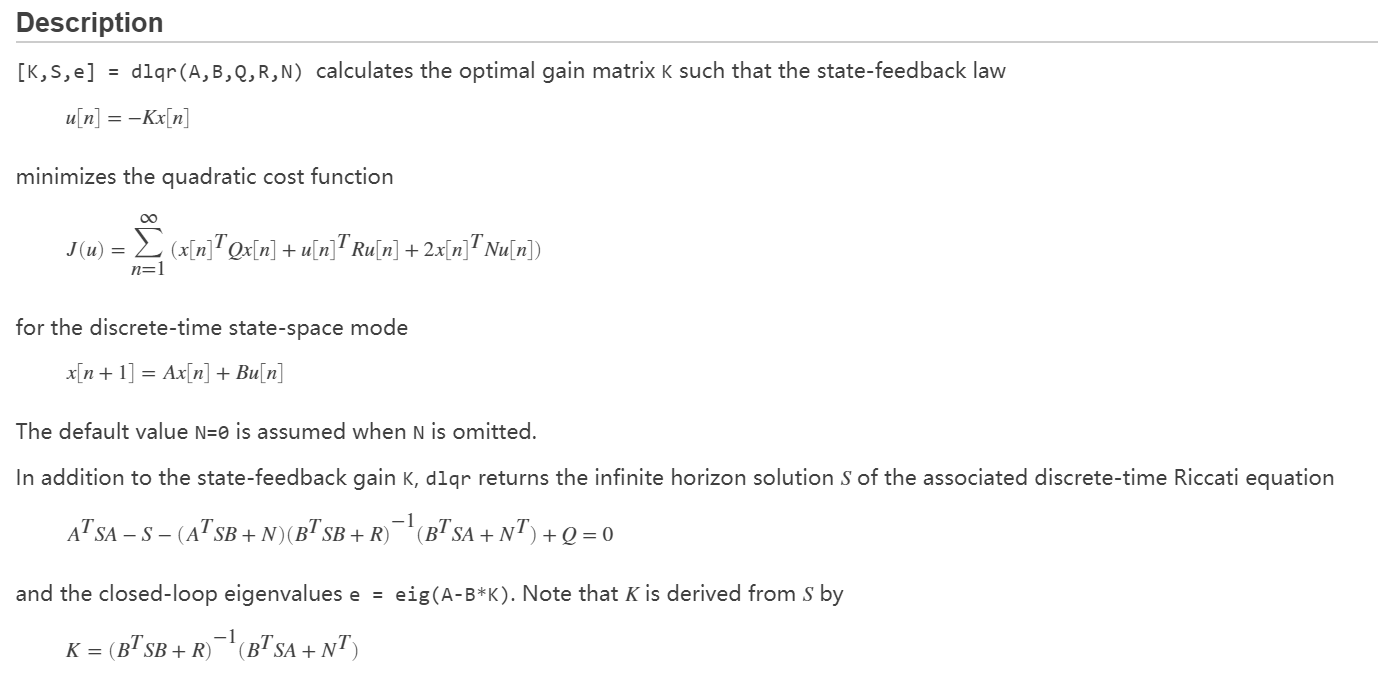
\includegraphics[width=\columnwidth]{Optimal Control of a Linear Discrete System/MCM20200128/picture/DLQR.png} %插入图片,[]中设置图片大小,{}中是图片文件名
  \label{Fig.RNN} %用于文内引用的标签
\end{figure}

\subsection{Dynamic Programming}
The final general characteristic of the dynamic-programming approach is the development of a recursive optimization procedure, which builds to a solution of the overall N-stage problem by first solving a one-stage problem and sequentially including one stage at a time and solving one-stage problems until the overall optimum has been found. This procedure can be based on a backward induction process, where the first stage to be analyzed is the final stage of the problem and problems are solved moving back one stage at a time until all stages are included. Alternatively, the recursive procedure can be based on a forward induction process, where the first stage to be solved is the initial stage of the problem and problems are solved moving forward
one stage at a time, until all stages are included. In certain problem settings, only one of these induction processes can be applied (e.g., only backward induction is allowed in most problems involving uncertainties).

The basis of the recursive optimization procedure is the so-called principle of optimality, which has already been stated: an optimal policy has the property that, whatever the current state and decision, the remaining decisions must constitute an optimal policy with regard to the state resulting from the current decision.

Suppose we have a multistage decision process where the return (or cost) for a particular stage is:

$$f_n(d_n,s_n)$$

where dn is a permissible decision that may be chosen from the set Dn, and sn is the state of the process with n stages to go.

Noramlly, we have to solve the following problem:

\[
v_{n}\left(s_{n}\right)=\operatorname{Max}\left[f_{n}\left(d_{n}, s_{n}\right)+f_{n-1}\left(d_{n-1}, s_{n-1}\right)+\cdots+f_{0}\left(d_{0}, s_{0}\right)\right]
\]
subject to:
\[
\begin{array}{ll}
s_{m-1}=t_{m}\left(d_{m}, s_{m}\right) & (m=1,2, \ldots, n) \\
d_{m} \in D_{m} & (m=0,1, \ldots, n)
\end{array}
\]

The generally cost-to-go function is:
$$J(f, x(t))=\min _{u(t) \in U}\left\{h(x(\tau))+\int_{t}^{T} g(x(\tau) \cdot u(\tau)) d \tau\right\}$$
\subsubsection{HJB function}:

And for this problem:
$$\begin{array}{l}
\left.\min x^{\top}(\tau) Q_{\tau} x(\tau)+\int_{0}^{\top}[x^T(\tau) Q x(\tau)+{u^T}(\tau) \operatorname{R u(\tau)}\right] d t \\
s .t. \quad {x}(t)=A x(t)+B a(t)
\end{array}$$

Define this problem's HJB function:
$$O=\min _{u(t) \in U} \left\{x^{\top} Q x+u^{\top} R u+x^{\top} k(t) x+2 x^{\top} k(t) 4 x+2 x^{\top} k(t) | 3 a\right\}$$

Derivative  it by u and let differential coefficient equals to zero:
$$2 R u+2 B^{T} k(t) x=0$$

Bring it back to HJB function:

$$O=x^{\top}(\left\{k(t)+k(t) A+A^Tk(t)-k(t) B R^{-1} B^{\top}k(t)\}\right )x$$

So we get Ricati Eqaution.

\subsubsection{Use HJB to solve this problem}

Define the weight matrix D:

$$D=diag(d_1,d_2...d_n)$$

With the restruct of u (because in the real world we don't have unlimited power to control)
$$g(u)=a u+b \leqslant 0$$
$Notes$: This function is the general condition for:
$$u_{min} \leqslant u \leqslant u_{max}$$

And for di:
$$\mathrm{d} i=\left\{\begin{array}{ll}
>0 & \mathrm{g}_{\mathrm{i}}(\mathrm{u})>0 \\
0 & \mathrm{g}_{\mathrm{i}}(\mathrm{u}) \leqslant 0
\end{array}\right.$$

So we expand the cost function:
$$\tilde{J}=\frac{1}{2} x^{T}\left(t_{0}\right) F_{x}\left(t_{0}\right)+-\frac{1}{2}-\int_{t}^{t}(  x^T Q(t)x+u^T R(t)u +g^T(u)Dg(u) )$$

For $\tilde{J}$, introduce the HJB funtion:

$$\begin{array}{l}
\widetilde{H}=-\frac{1}{2}-\mathrm{X}^{\mathrm{T}}\left(2(\mathrm{t}) \mathrm{x}+\frac{1}{2} \mathrm{u}^{\mathrm{T}} \mathrm{R}(t) \mathrm{u}+\right. \\
-\frac{1}{2} \mathrm{g}^{\mathrm{T}}(\mathrm{u}) \mathrm{Dg}(\mathrm{u})+\lambda^{\mathrm{T}} \mathrm{A}(\mathrm{x}) \mathrm{x}+\lambda^{\mathrm{T}} \mathrm{B}(\mathrm{t}) \mathrm{u}
\end{array}$$
where $\lambda$ is Lagrange multiplier.

Using maximum principle we can get $u^{*}(t)$:
$$u^{*}=-\tilde{R}^{-1}(t)\left[B^{T}(t) \lambda+\tilde{b}\right]$$
where:
$$\begin{array}{c}
\widetilde{R}(t)=R(L)+a^{\prime} D a>0 \\
\widetilde{b}=a^{\prime} D b
\end{array}$$

%%%此处很多没看懂,已高亮
$$\begin{array}{c}
\dot{x}=A(t) x-B(t) \widetilde{R}^{-1}(t) B^T(t) \lambda 
-B(t) \widetilde{R}^{-1}(t) \widetilde{b}
\end{array} $$
Suppose:
$$\lambda=P(t) x+P_0(t)$$
Here:
$$P \in R^{n \times n},  P_{0} \in R^{n \times 1}$$
Put it in to $\lambda$ can get:
$$\dot{\lambda}=\dot{P}(t) x+P(t) \dot{x}+\dot{P}_{0}(t)$$

Finally we get:
\begin{align}\dot{\lambda}=[\dot{\mathrm{P}}(\mathrm{t})+\mathrm{P}(\mathrm{t}) \mathrm{A}(\mathrm{t})-\mathrm{P}(\mathrm{t}) \mathrm{B}(\mathrm{t}) 
\left.\widetilde{\mathrm{R}^{-1}}(\mathrm{t}) \mathrm{PB}^{\mathrm{T}}(\mathrm{t})(\mathrm{t})\right] \mathrm{x}-\\P(\mathrm{t}) \mathrm{B}(\mathrm{t})
\widetilde{\mathrm{R}}^{-1} 
(\mathrm{t}) \mathrm{B}^{\mathrm{r}}(\mathrm{t}) \mathrm{P}_{\mathrm{o}}(\mathrm{t})-\mathrm{P}(1) \mathrm{B}(\mathrm{t}) \mathrm{R}^{-1} 
(\mathrm{t}) \tilde{\mathrm{b}}+\dot{\mathrm{P}}_{\mathrm{o}}(\mathrm{t})
\end{align}

We also have:
\begin{align}
\dot{\lambda}=&-\left[\mathrm{Q}(\mathrm{t})+\mathrm{A}^{\mathrm{T}}(\mathrm{t}) \mathrm{P}(\mathrm{t})\right] \mathrm{x} 
-\mathrm{A}^{\mathrm{T}}(\mathrm{t}) P_0^T(\mathrm{t})
\end{align}

Compare (13-14) and (15) we can get:

\begin{align}
\dot{\mathrm{P}}(\mathrm{t})=&-\mathrm{A}^{T}(\mathrm{t}) \mathrm{P}(\mathrm{t})-\mathrm{P}(\mathrm{t}) \mathrm{A}(\mathrm{t})+\mathrm{P}(\mathrm{t}) \mathrm{B}(\mathrm{t}) \widetilde{\mathrm{R}}^{-1}(\mathrm{t}) \mathrm{B}^{\mathrm{T}}(\mathrm{t})  \mathrm{P}(\mathrm{t})-\mathrm{Q}(t)
\end{align}

And

\begin{align}
\dot{P}_{o}(t)=&-G^{T}(t) P_{0}(t)+P(t) B(t) \widetilde{\mathrm{R}}^{-1}(t) \vec{b} 
\end{align}
where: $G(t)=A(t)-B(t) \widetilde{\mathrm{R}}^{-1}(t) B^{T}(t) P^T(t)$

Due to $\widetilde{\mathrm{R}},\widetilde{\mathrm{P}}$ are symmetric matrix:

$$G^T(t)=A^{T}(t)-P(1) B(t) \widetilde{R}^{-1}(1) B^{T}(t)$$


%%%%%%%%%%%%%%%%%%%%%%%%%%%%%%
%%%%%%%%%%%%%%%%%%%%%%%%%%%%%%%
%%%%%%%%%%%%%%%%%%%%%%%%%%%%


\section{The Comprehensive Evacuation Planning Model}
\subsection{Model Preparation}

\begin{itemize}

\item Station nodes: In this problem, the locations of all station nodes are known and fixed, and the demand generation changes over time to meet the S type behavior curve. Requirements may exceed the load capacity of the vehicle during the process of time change. In this case, it may be necessary to mobilize the vehicle from other station nodes or carry out the second transport. Having no time limit on the vehicle service, evacuees can be carried out at any time in station nodes, and the transport vehicle is set at the set point;
\item Transport vehicle: In this problem, all vehicles start from the shelter, via the station node, and then complete the transport mission, during which the overload operation is not allowed to exceed the maximum driving time of the vehicle;

\item Shelter: In this problem, there are several shelters whose location and capacity have been determined.
\end{itemize}

VRP \cite{Dikas2016Solving,He2015Model} generally defined as: on a range of clients point (location known or can be estimated) in satisfying certain constraints (such as the demand for goods, the delivery time of delivery, the vehicle capacity constraints, etc.), reasonably arrange the vehicle distribution route, making the vehicle through them in an orderly way to achieve a certain goal (such as the shortest mileage and least cost, least time, use as little as possible and so on). The representation of VPR can be seen in Figure 3.

\begin{figure}[tbp]
  \centering{
  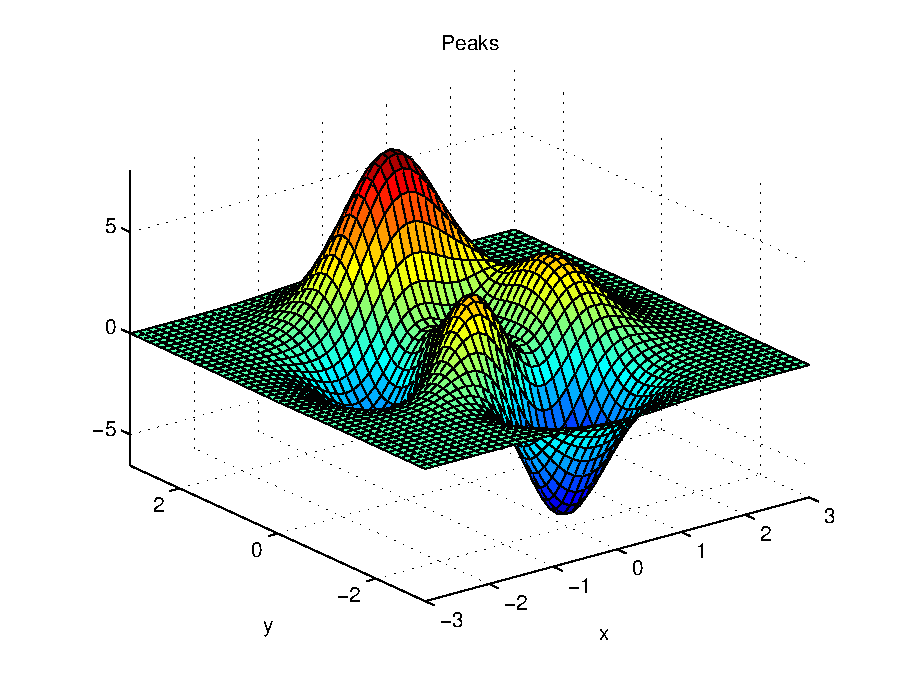
\includegraphics[width=0.7\textwidth]{./picture/figure3.eps}}
  \caption{A Typical Vehicle Routing Problem}\label{Figure3}
\end{figure}

Based on the traditional VRP, a comprehensive evacuation planning model is established to satisfy the constraint conditions:
\begin{itemize}
  \item Time constraint: the total withdrawal time is the shortest in the case of meeting all the evacuees' needs and not violating the constraints;
  \item Risk constraint: minimum risk of meeting the minimum evacuation time;
  \item Carrying capacity constraint: the number of customers on each vehicle path is limited no more than a constant;
  \item Road afford ability constraint: the total carrying capacity on the road is not allowed to exceed the road capacity;
  \item Shelter capacity constraint: the total population in the shelter shall is not allowed to exceed the capacity limit;
  \item Priority relationship constraints: the more endangered areas have priority access;
  \item Path first constraint: after every vehicle completes its mission, records its shelter and the time to reach the sanctuary, preparing for the assignment of the next mission.
\end{itemize}

Before each task, we need to update the network node demand, shelter of residual capacity and the starting position of the vehicles, where each task should be according to the last mission at the end of the vehicle at the beginning of status to the caller, get the transport vehicles in the task.

\subsection{Modeling}

We now describe an optimization model that includes the assumptions of the previous section %%\cite{Goerigk2014Combining}.

The considered time horizon is denoted by $T$. This is not the evacuation time we are aiming for, but an upper bound on the evacuation time that is needed by our model. This quantity is used to build the time expanded network.

For public transportation we assume that there is already an established set of collection points, where evacuees gather for further transportation to shelters. For each collection point it is known how many people will appear at this point in each time step. We also given a set of possible shelter location. For each such location we are given the number of people ${W_j}$ that this shelter can hold and additionally the parking space ${C_j}$ available near this shelter.

The set of buses available for the public evacuation transit is denoted by B. For simplicity, we assume that all buses have the same capacity ${N_0}$ (however, different capacities can easily be included in our model). Besides all cars carry the same number of people.

Once the used shelter locations have been chosen, the public and private traffic will pour into the shelter. The private traffic is modeled as a dynamic network flow, the public traffic (the buses) as a dynamic multi commodity network flow. The private traffic is a single commodity whereas each bus is a commodity of its own. The flow of the buses has to be chosen such that all people that need public transportation can be brought to shelter locations while respecting the bus capacity. Both flows are chosen simultaneously in a system optimal way.

The total risk exposure is given by the sum of the risks of the individual arcs over all time steps. The risk of a single arc at a time step is given by the risk value of the arc multiplied with the number of people on this arc at this time step.

Formulating these aspects mathematically, we propose the following multi-criteria mixed-integer programming model, which we call the Comprehensive Evacuation Problem (CEP)\cite{Murray2013Evacuation,Ng2015Sharp,Ng2010Reliable}

In this mixed integer program we use the following variables: $\delta _{ij}$ denotes traversal of arc (i,j) $ \in $ A. $x_{ij}^t$ denotes the spend time passing arc (i,j). $r_{ij}^t$ denotes the risk factor passing arc (i,j) at time $t$. $f_{ij}^t$ denotes the number of evacuees using cars passing arc (i,j) at time $t$. In contrast, $g_{ij}^t$ denotes the number of evacuees using bus $b$ to go from node $i$ to node $j$ at time $t$. $\eta $ represents the jam factor, which depends on the magnitude of the hurricane, the location of the landing, and the average number of evacuees passing arc (i,j) at time $t$. $B_{ij}^t$ denotes the number of bus driving on arc (i,j) at time $t$.In the same way, $C_{ij}^t$ denotes the number of car driving on arc (i,j) at time $t$. $P_j^t$  denotes the number of people in the $j$ shelter at time $t$. $r$ denotes the capacity factor.


\begin{equation}\label{3}
\Delta \min (\Delta ,R)
\end{equation}

\begin{equation}\label{4}
\Delta  \ge (2n - 1) \times \max (\sum\limits_{(i,j) \in A} {\sum\limits_{t \in T} {\delta _{ij}^tx_{ij}^t} } ) + \Delta t
\end{equation}

The objective (1) is to minimize the evacuation time $\Delta $ and the risk $R$ ,These objectives are computed using constraints (2)-(4). Constraints (2) ensure that $\Delta $ is the maximal evacuation time. The risk $R$ depends on the number of people passing a link. This relation is expressed in constraint (3)and(4).

\begin{equation}\label{5}
 R = \sum\limits_{(i,j) \in A} {\sum\limits_{t \in T} {r_{ij}^t} } (f_{ij}^t + \sum\limits_{(i,j) \in A} {{\rm{g}}_{ij}^t} ) + W + V
\end{equation}

\begin{equation}\label{6}
\sum\limits_{(i,j) \in A} {\sum\limits_{t \in T} {f_{ij}^t} }  = {N_i} \times a\%
\end{equation}

\begin{equation}\label{7}
n = \left[ {\frac{{{N_{\rm{i}}} \times (1 - a\% )}}{{{B_i} \times {N_0}}}} \right]{\rm{ + }}1
\end{equation}

\begin{equation}\label{8}
x_{ij}^t = \eta \frac{{{S_{ij}}}}{{{v_b}}}
\end{equation}

\begin{equation}\label{9}
{\rm{g}}_{ij}^t = {N_0} \times B_{ij}^t
\end{equation}

\begin{equation}\label{10}
C_{ij}^t{\rm{ = p}} \times {{\rm{C}}_i}
\end{equation}

In the equation (5), $n$ means the number of journeys that the bus needs to transport, and the calculation should Integer plus one. Equation (8) - (10) is the road traffic that is used to constrain not to exceed its maximum capacity at time $t$.

\begin{equation}\label{11}
B_{ij}^t = {\rm{p}} \times {{\rm{B}}_i}
\end{equation}

\begin{equation}\label{12}
C_{ij}^t + B_{ij}^t \le {V_{ij}}
\end{equation}

The individual and the public traffic are linked together in the edge capacity constraints (11)-(12). Each used shelter must supply enough parking space and enough room to support evacuees.

\begin{equation}\label{13}
C_j^t \le {C_j}
\end{equation}

\begin{equation}\label{14}
P_j^t \le r{W_j}
\end{equation}

\begin{equation}\label{15}
r = \frac{{{N_{\rm{i}}}}}{{{W_j}}}
\end{equation}

When a hurricane is stronger, it may require a massive evacuation, that is, to consider the interaction of the three states. The site selection, risk coefficient, road congestion, and site accommodation will be affected, we need to reset the influence parameters to get the minimum required time and the site situation again.

Optimization method: When the forecast hat hurricane level is high, we can arrange inland evacuation ahead, in the case of ensure the overall time is enough for the coastal areas to evacuate to the site of the corresponding time calculation.

Advantage: Inland remove first can reduce the road pressure; Coastal remove later can increase the economic benefit.Compare the results again and get the final optimization plan.

\subsection{Model Solution}
Based on the above model and the parameters involved in the model, the final evacuation time is obtained by programming, and the result is shown in the table below:
\begin{table}[!htb]
\centering
\setlength{\abovecaptionskip}{0pt}%    
\setlength{\belowcaptionskip}{10pt}%
\caption{The Evacuation time}
\begin{tabular}{ccccccc}
\toprule[1.5pt]
Hurricane level &1&2&3&4&5&6\\
Evacuation time &11.4&18.2&24.28&33.6&47.8&49.6\\
\bottomrule[1.5pt]
\end{tabular}
\end{table}
%\begin{figure}[h]
%  \centering{
%  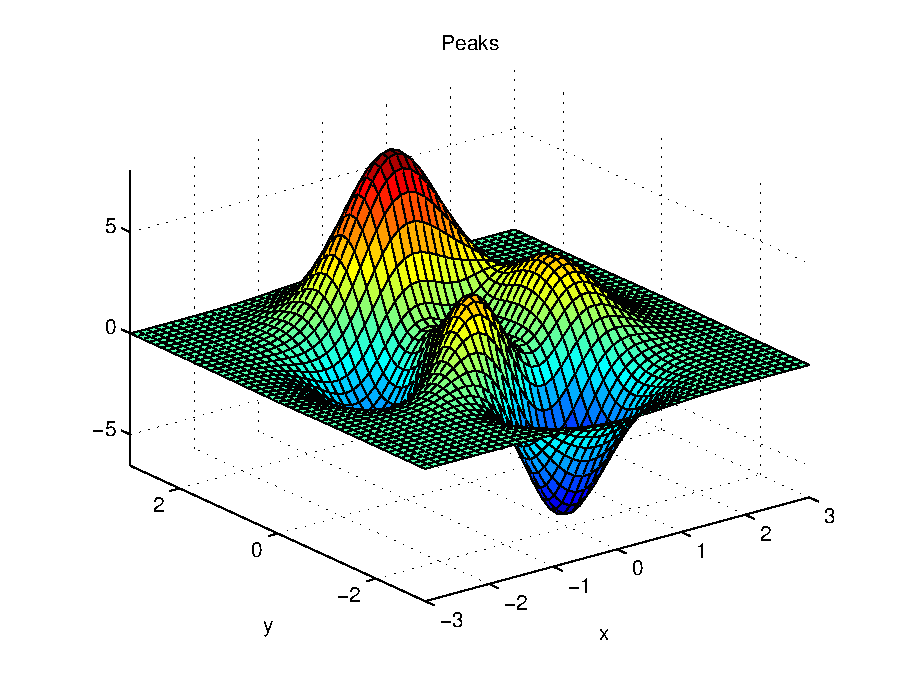
\includegraphics[width=0.7\textwidth]{./picture/figure4.eps}}
%  \caption{The Evacuation Time}\label{Table1}
%\end{figure}



As shown in the figure above, it is necessary to calculate the time required for a category 1- 5 hurricane, including the withdrawal time required for the optimization programme.

Because the evacuation and time of personnel also satisfied the curve of $S$ type curve, it can be used to draw the time-varying personnel evacuation curve of hurricane from category 1 - 5, which can be seen in figure4.

\begin{figure}[h]
  \centering{
  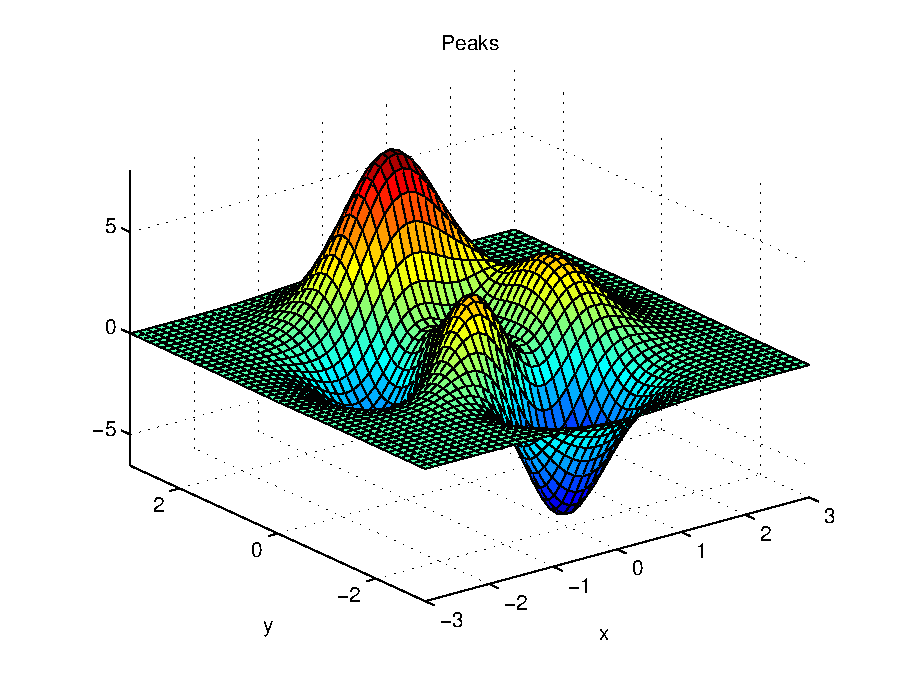
\includegraphics[width=0.7\textwidth]{./picture/figure5.eps}}
  \caption{The time-varying personnel evacuation curve of hurricane from category 1 - 5}\label{figure4}
\end{figure}

On the basis of guarantee the safety of life, we put forward the optimization scheme, when hurricane prediction level too high, let let evacuated inland areas, in order to improve the economic benefit of coastal, and reduce economic loss. The maximum population density due to coastal areas, and abide by the $S$ type curve evacuation rules.

\begin{figure}[h]
  \centering{
  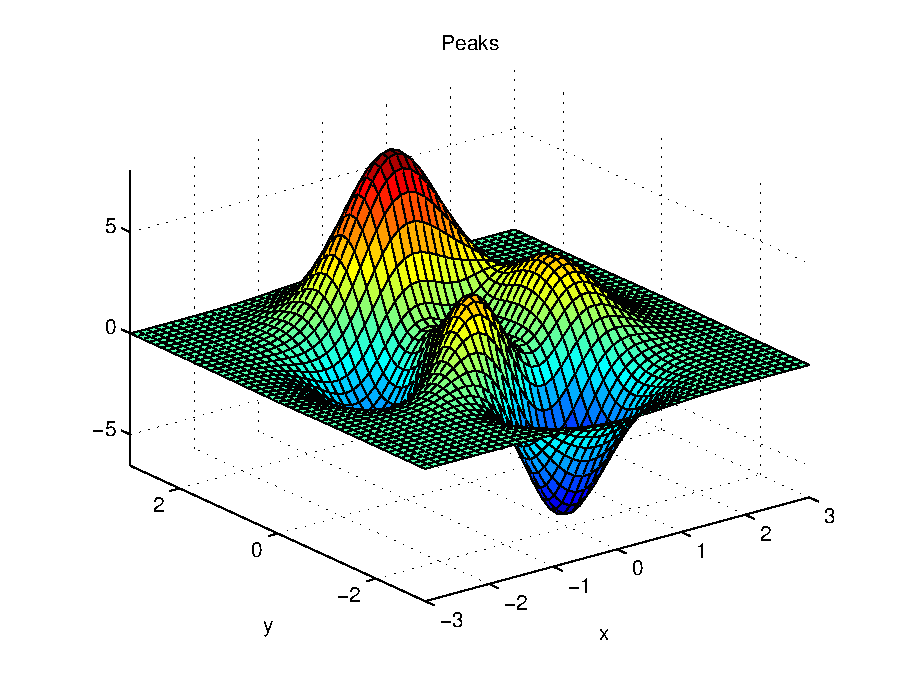
\includegraphics[width=0.7\textwidth]{./picture/figure6.eps}}
  \caption{Optimize personnel evacuation curve}\label{figure5}
\end{figure}

Under the same Five - level hurricane conditions, the optimization scheme minimizes the economic loss under the conditions of increasing the cost of the smaller time. It has been proved that evacuating in the right time can get better effect, which has a positive effect on the subsequent development of evacuation plan.

\section{Strengths and Weaknesses}

\subsection{Strengths}

\begin{itemize}
  \item The comprehensive evacuation planning model takes the shortest time and lowest risk and low economic losses as the total constraint conditions to get the optimal solution;
  \item The constraint conditions such as road carrying capacity and the capacity of escape points are considered in the comprehensive evacuation planning model;
  \item Determine the coverage scope by Thiessen polygon;
  \item Considering the demand distribution characteristics in the station nodes;
  \item In terms of model constraints, the shortest evacuation time is obtained for a 1-5 hurricane;
  \item Considering the economic benefit gap between inland and coastal areas, the optimal plan for economic loss is proposed;
  \item Analyze the extreme problems, propose solutions, and obtain the optimal solution through comprehensive consideration of evacuation time, evacuation risks and economic losses.
\end{itemize}

\subsection{Weaknesses and Extensions}
\begin{itemize}
  \item Without considering the evacuation of the county itself;
  \item Without considering the refueling problem of cars and buses;
  \item Without considering the risk caused by large numbers of people in station nodes;
  \item Without considering other means of transportation, such as aircraft, railway, etc.;
  \item Without considering the subsequent material problems of the shelter.
\end{itemize}

Optimization method: When the forecast hat hurricane level is high, we can arrange inland evacuation ahead, in the case of ensure the overall time is enough for the coastal areas to evacuate to the site of the corresponding time calculation.

Advantage: Inland remove first can reduce the road pressure; Coastal remove later can increase the economic benefit. Compare the results again and get the final optimization plan.

\addcontentsline{toc}{section}{Reference}
\bibliographystyle{plain}
\bibliography{myreference}

\begin{appendices}

\section{First appendix}

In addition, your report must include a letter to the Chief Financial Officer (CFO) of the Goodgrant Foundation, Mr. Alpha Chiang, that describes the optimal investment strategy, your modeling approach and major results, and a brief discussion of your proposed concept of a return-on-investment (ROI). This letter should be no more than two pages in length.

\begin{letter}{Dear, Mr. Alpha Chiang}

\lipsum[1-2]

\vspace{\parskip}

Sincerely yours,

Your friends

\end{letter}
Here are simulation programmes we used in our model as follow.\\

\textbf{\textcolor[rgb]{0.98,0.00,0.00}{Input matlab source:}}
\lstinputlisting[language=Matlab]{./code/mcmthesis-matlab1.m}

\section{Second appendix}

some more text \textcolor[rgb]{0.98,0.00,0.00}{\textbf{Input C++ source:}}
\lstinputlisting[language=C++]{./code/mcmthesis-sudoku.cpp}

\end{appendices}
\end{document}
